\documentclass[12pt,fleqn,handout]{beamer}


\xdefinecolor{lavendar}{rgb}{0.8,0.6,1}
\xdefinecolor{olive}{cmyk}{0.64,0,0.95,0.4}
%\xdefinecolor{olive}{cmyk}{1,0,0,0}
\xdefinecolor{mag}{cmyk}{0.1,1,0,0.2}
\xdefinecolor{lblue}{rgb}{0,0,1.5}
\xdefinecolor{lred}{rgb}{1,0,0}
\xdefinecolor{mine}{cmyk}{1,0,0.2,0}
\xdefinecolor{bluel}{cmyk}{0.1,0,0.9,0.4}

\usepackage{amsmath,amssymb,dsfont,mathrsfs}
\usepackage{tikz,pgflibraryplotmarks}
\usepackage{multimedia}
\usepackage{wasysym}
\usepackage{rotating}
\usepackage{algorithm,algorithmic}
\usepackage{graphicx} % more modern
\usepackage{subfigure}
\usepackage{booktabs}

\usepackage{pgfplots}
\usepackage{verbatim}

\usepackage{setspace}
\newlength\iwidth
\newlength\iheight

\newcommand\makebeamertitle{\frame{\maketitle}}%
\graphicspath{{./images/}}
\setbeamertemplate{navigation symbols}{}
\addtobeamertemplate{navigation symbols}{}{%
    \usebeamerfont{footline}%
    \usebeamercolor[fg]{footline}%
	\insertshorttitle
    \;--
    \insertframenumber
}

\newcommand{\sectionstart}{
	\only<beamer>{
 	\begin{frame}% (fold)
 		\begin{centering}\Huge \insertsection \par\end{centering}
 	\end{frame}% frame the_application (end)
	}
 }


% make bibliography entries smaller
\usepackage{natbib}
\setbeamertemplate{bibliography item}{[\theenumiv]}
\renewcommand\bibfont{\scriptsize}
\setbeamertemplate{frametitle continuation}[from second]
\newcommand{\tcr}{\textcolor{red}}
\newcommand{\tcrd}{\textcolor{red}}
\newcommand{\tcb}{\textcolor{bluel}}
\newcommand{\tcm}{\textcolor{mag}}
\newcommand{\tcg}{\textcolor{olive}}

\newcommand{\R}{\mathbb{R}}
\newcommand{\C}{\mathbb{C}}

% bold lower-case for vectors
\newcommand{\bfa}{{\bf a}}
\newcommand{\bfb}{{\bf b}}
\newcommand{\bfc}{{\bf c}}
\newcommand{\bfs}{{\bf s}}
\newcommand{\bfm}{{\bf m}}
\newcommand{\bfd}{{\bf d}}
\newcommand{\bfe}{{\bf e}}
\newcommand{\bfu}{{\bf u}}
\newcommand{\bfy}{{\bf y}}
\newcommand{\bfx}{{\bf x}}
\newcommand{\bfh}{{\bf h}}
\newcommand{\bfw}{{\bf w}}
\newcommand{\bfv}{{\bf v}}
\newcommand{\bfr}{{\bf r}}
\newcommand{\bfz}{{\bf z}}
\newcommand{\bfp}{{\bf p}}


% bold upper-case for linear operators
\newcommand{\bfA}{{\bf A}}
\newcommand{\bfB}{{\bf B}}
\newcommand{\bfZ}{{\bf Z}}
\newcommand{\bfM}{{\bf M}}
\newcommand{\bfC}{{\bf C}}
\newcommand{\bfD}{{\bf D}}
\newcommand{\bfQ}{{\bf Q}}
\newcommand{\bfJ}{{\bf J}}
\newcommand{\bfG}{{\bf G}}
\newcommand{\bfI}{{\bf I}}
\newcommand{\bfP}{{\bf P}}
\newcommand{\bfK}{{\bf K}}
\newcommand{\bfY}{{\bf Y}}
\newcommand{\bfW}{{\bf W}}
\newcommand{\bfR}{{\bf R}}
\newcommand{\bfL}{{\bf L}}
\newcommand{\bfF}{{\bf F}}
\newcommand{\bfT}{{\bf T}}
\newcommand{\bfS}{{\bf S}}
\newcommand{\bfX}{{\bf X}}
\newcommand{\bfU}{{\bf U}}
\newcommand{\bfV}{{\bf V}}
\newcommand{\bfH}{{\bf H}}


\newcommand{\calF}{\mathcal{F}}



\newcommand{\hf}{{\frac 12}}
\newcommand{\bftheta}{{\boldsymbol \theta}}
\newcommand{\bfxi}{{\boldsymbol \xi}}

\newcommand{\bfLambda}{{\boldsymbol \Lambda}}
\newcommand{\bfSigma}{{\boldsymbol \Sigma}}
\newcommand{\bfepsilon}{{\boldsymbol \epsilon}}

\newcommand{\E}{\vec E}
\newcommand{\B}{\vec B}

\newcommand{\vu}{  {\vec {\bf u}}}

\newcommand{\grad}{  {\vec {\bf \nabla}}}

\newcommand{\lfrownie}{\textcolor{red}{\large{\frownie}}}
\newcommand{\lsmiley}{\textcolor{green}{\large{\smiley}}}

\newcommand{\curl}{\ensuremath{\nabla\times\,}}
\renewcommand{\div}{\nabla\cdot\,}
\newcommand{\divh}{\nabla_h\cdot\,}
\renewcommand{\grad}{\ensuremath{\nabla}}

\DeclareMathOperator*{\argmin}{arg\,min}


\title[Reg Image Class]{Regularization for Image Classification}
\subtitle{Numerical Methods for Deep Learning}
\date{}
\begin{document}

\makebeamertitle


\section{Regularization in Imaging} % (fold)
\label{sec:regularization_in_imaging}

\begin{frame}[fragile]\frametitle{Why use regularization?}
We are attempting to train weights $\bfW \in \R^{n_c \times n_f}$ to express the relation between some data $\bfY \in \R^{n_f \times n}$ and their labels $\bfC \in \R^{n_c \times n}$ by solving
$$
	 \min_\bfW  E(\bfW) =  E(\bfC,\bfW,\bfY)
$$ 
Recall: ${\rm rank}(\bfY) \leq \min\{n_f,n\}$
\begin{itemize}
\item $n < n_f$: No unique solution
\item $n > n_f$: $\bfY$ may still be rank-deficient
\end{itemize}

\pause

Challenges in image classification: 
\begin{itemize}
	\item data is high dimensional ($n_f \approx$ number of pixels/voxels/frames)
	\item higher resolution $\leadsto$ need more examples? 
	\item higher resolution $\leadsto$ larger rank?
\end{itemize}

\end{frame}


\begin{frame}[fragile]\frametitle{Regularization}
If Hessian $\nabla^2 E$ highly ill-conditioned, regularization is needed.
\begin{itemize}
\item Symptom: weights are large or oscillatory.
\item Alternative: Estimate condition number (costly!)
\end{itemize}

\pause

Solution: require solution to be regular
$$ \min_W\ \phi(\bfW) = E(\bfW) + \lambda R(\bfW), $$

where
\begin{itemize}
	\item $R$ is a regularizer, $R(\bfW)$ large when $\bfW$ is irregular and small otherwise
	\item $\lambda$ is a regularization parameter (needs to be chosen)
	\item Mathematically: $R$ makes sure $\bfW^*$ lies in desired function space (and is sufficiently \emph{regular}).
\end{itemize}

Excellent references include~\cite{Hansen1998,Hansen2010, Vogel2002}.
\end{frame}


\begin{frame}
	\frametitle{What is an Image?}
	
	\begin{center}
		\begin{tabular}{cc}
			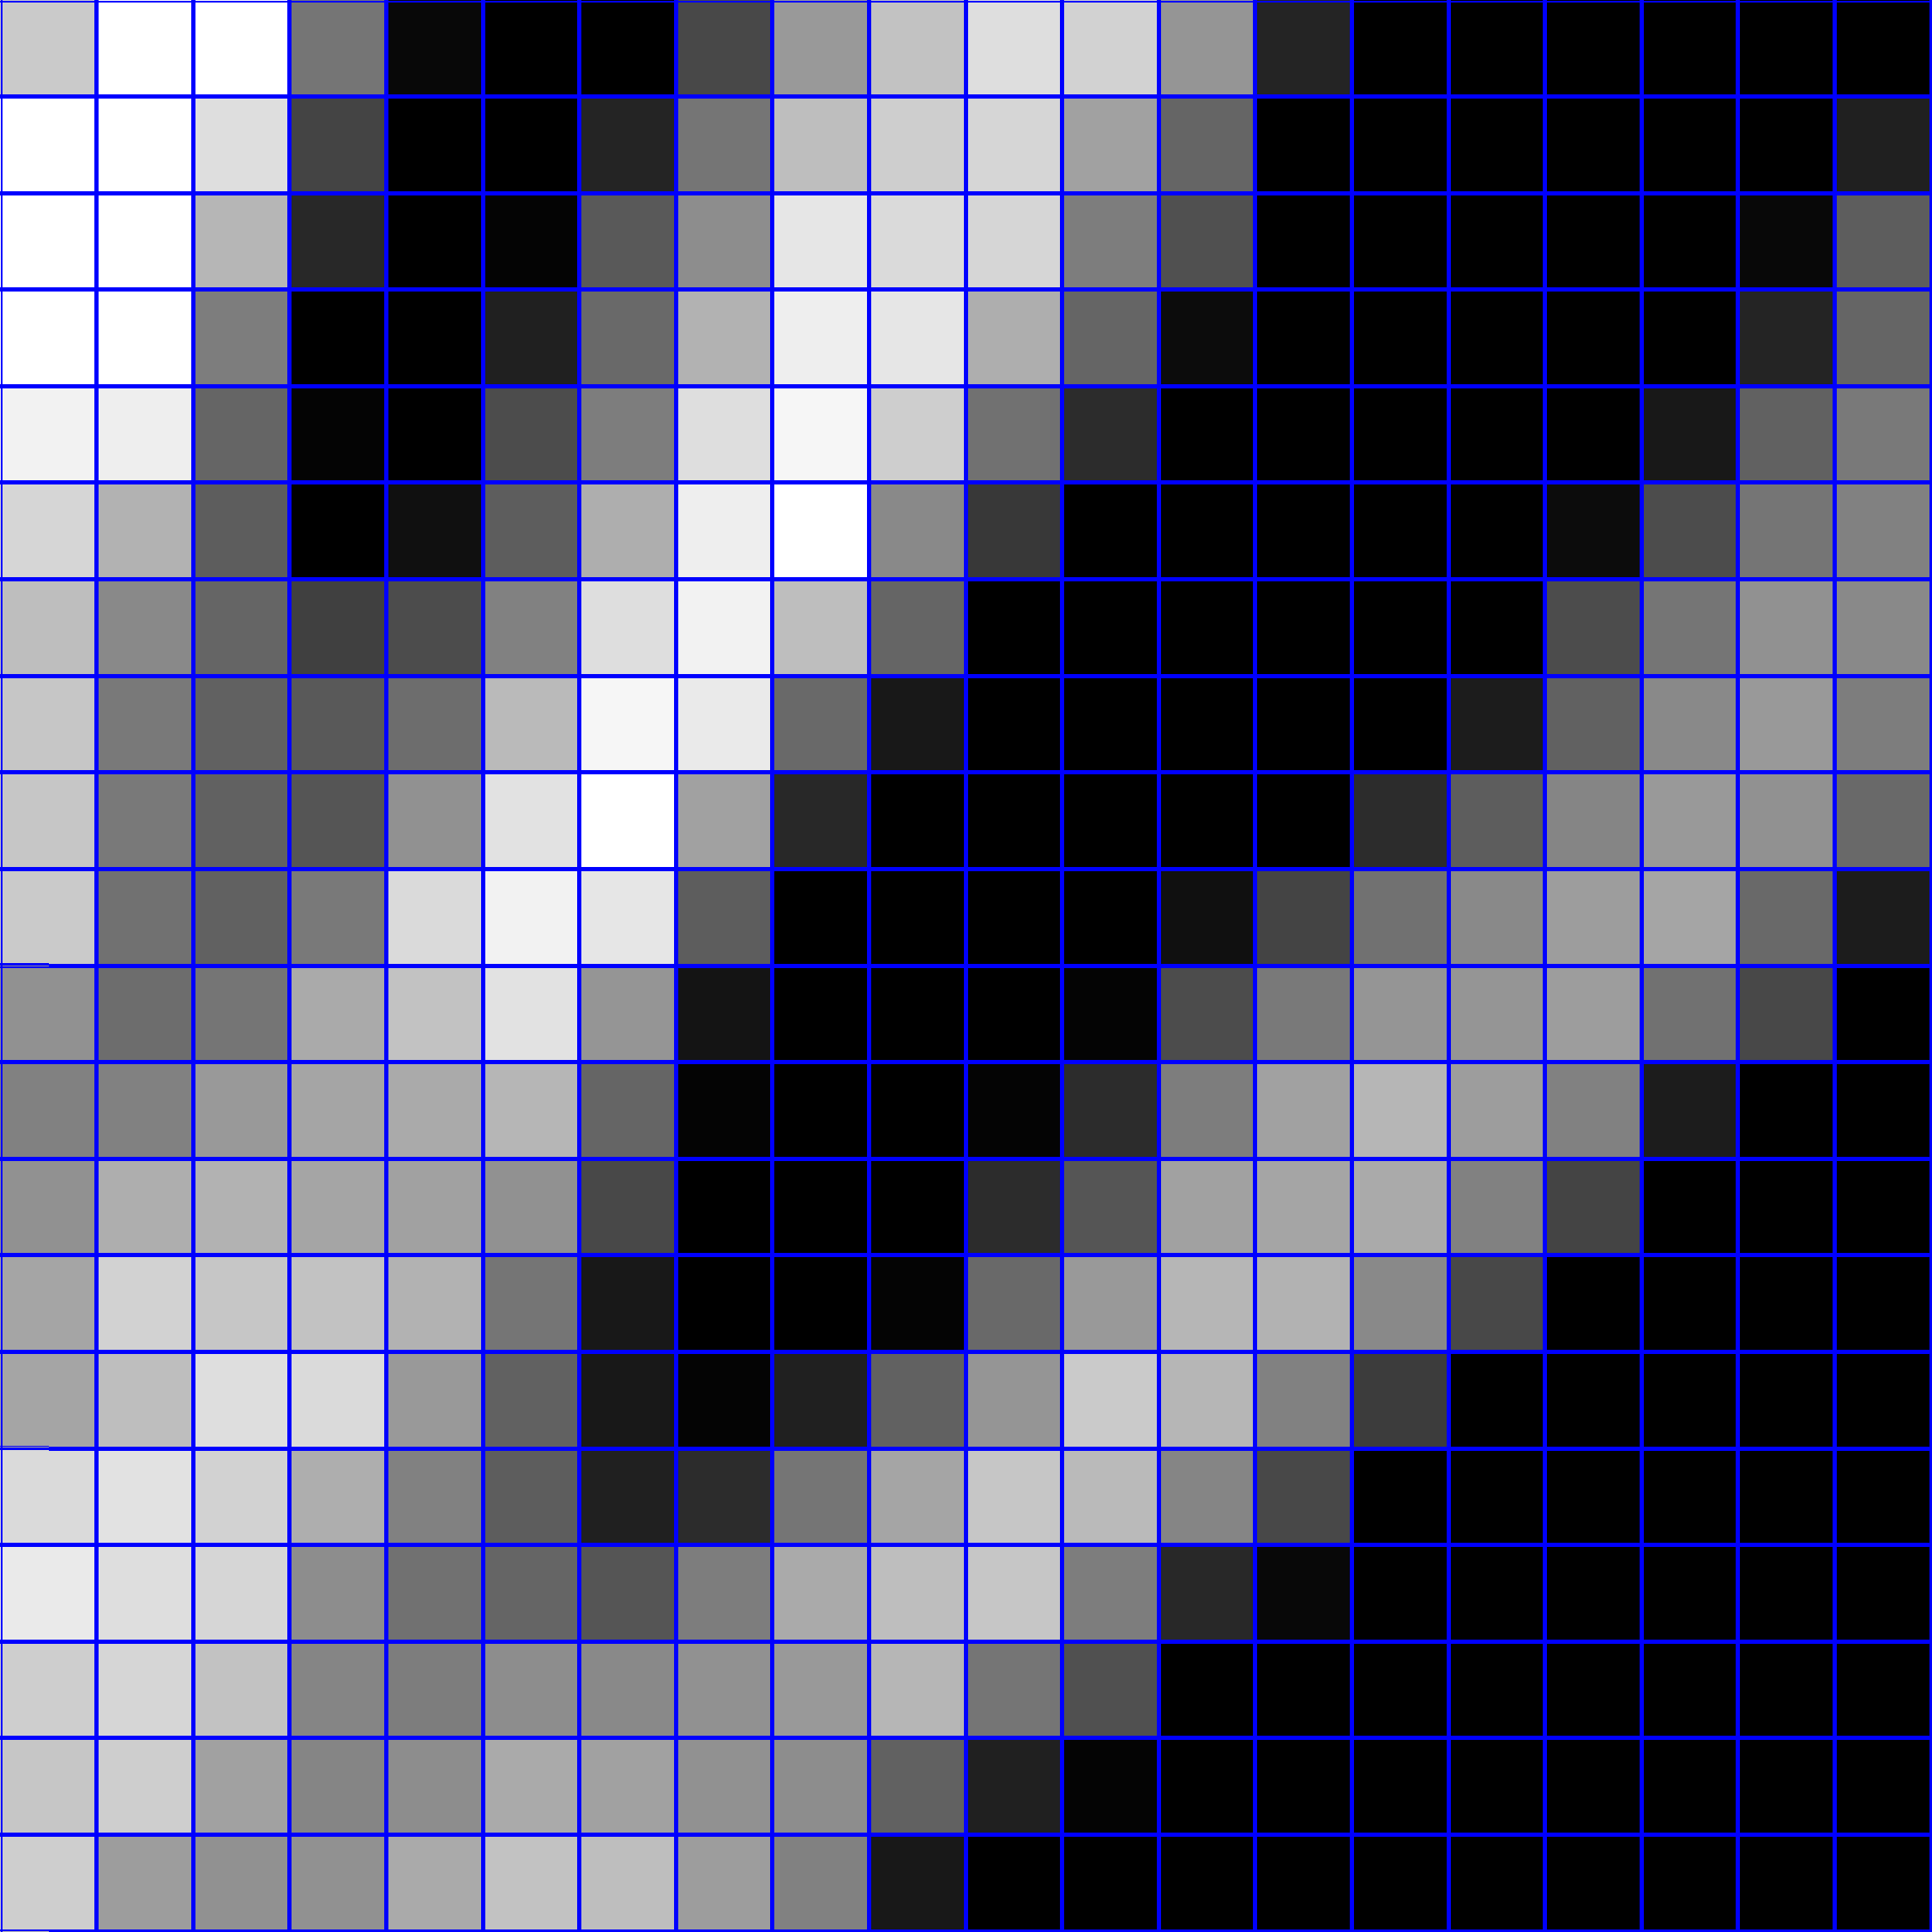
\includegraphics[width=30mm]{image-model2D-data}
			&
			\invisible<beamer|1>{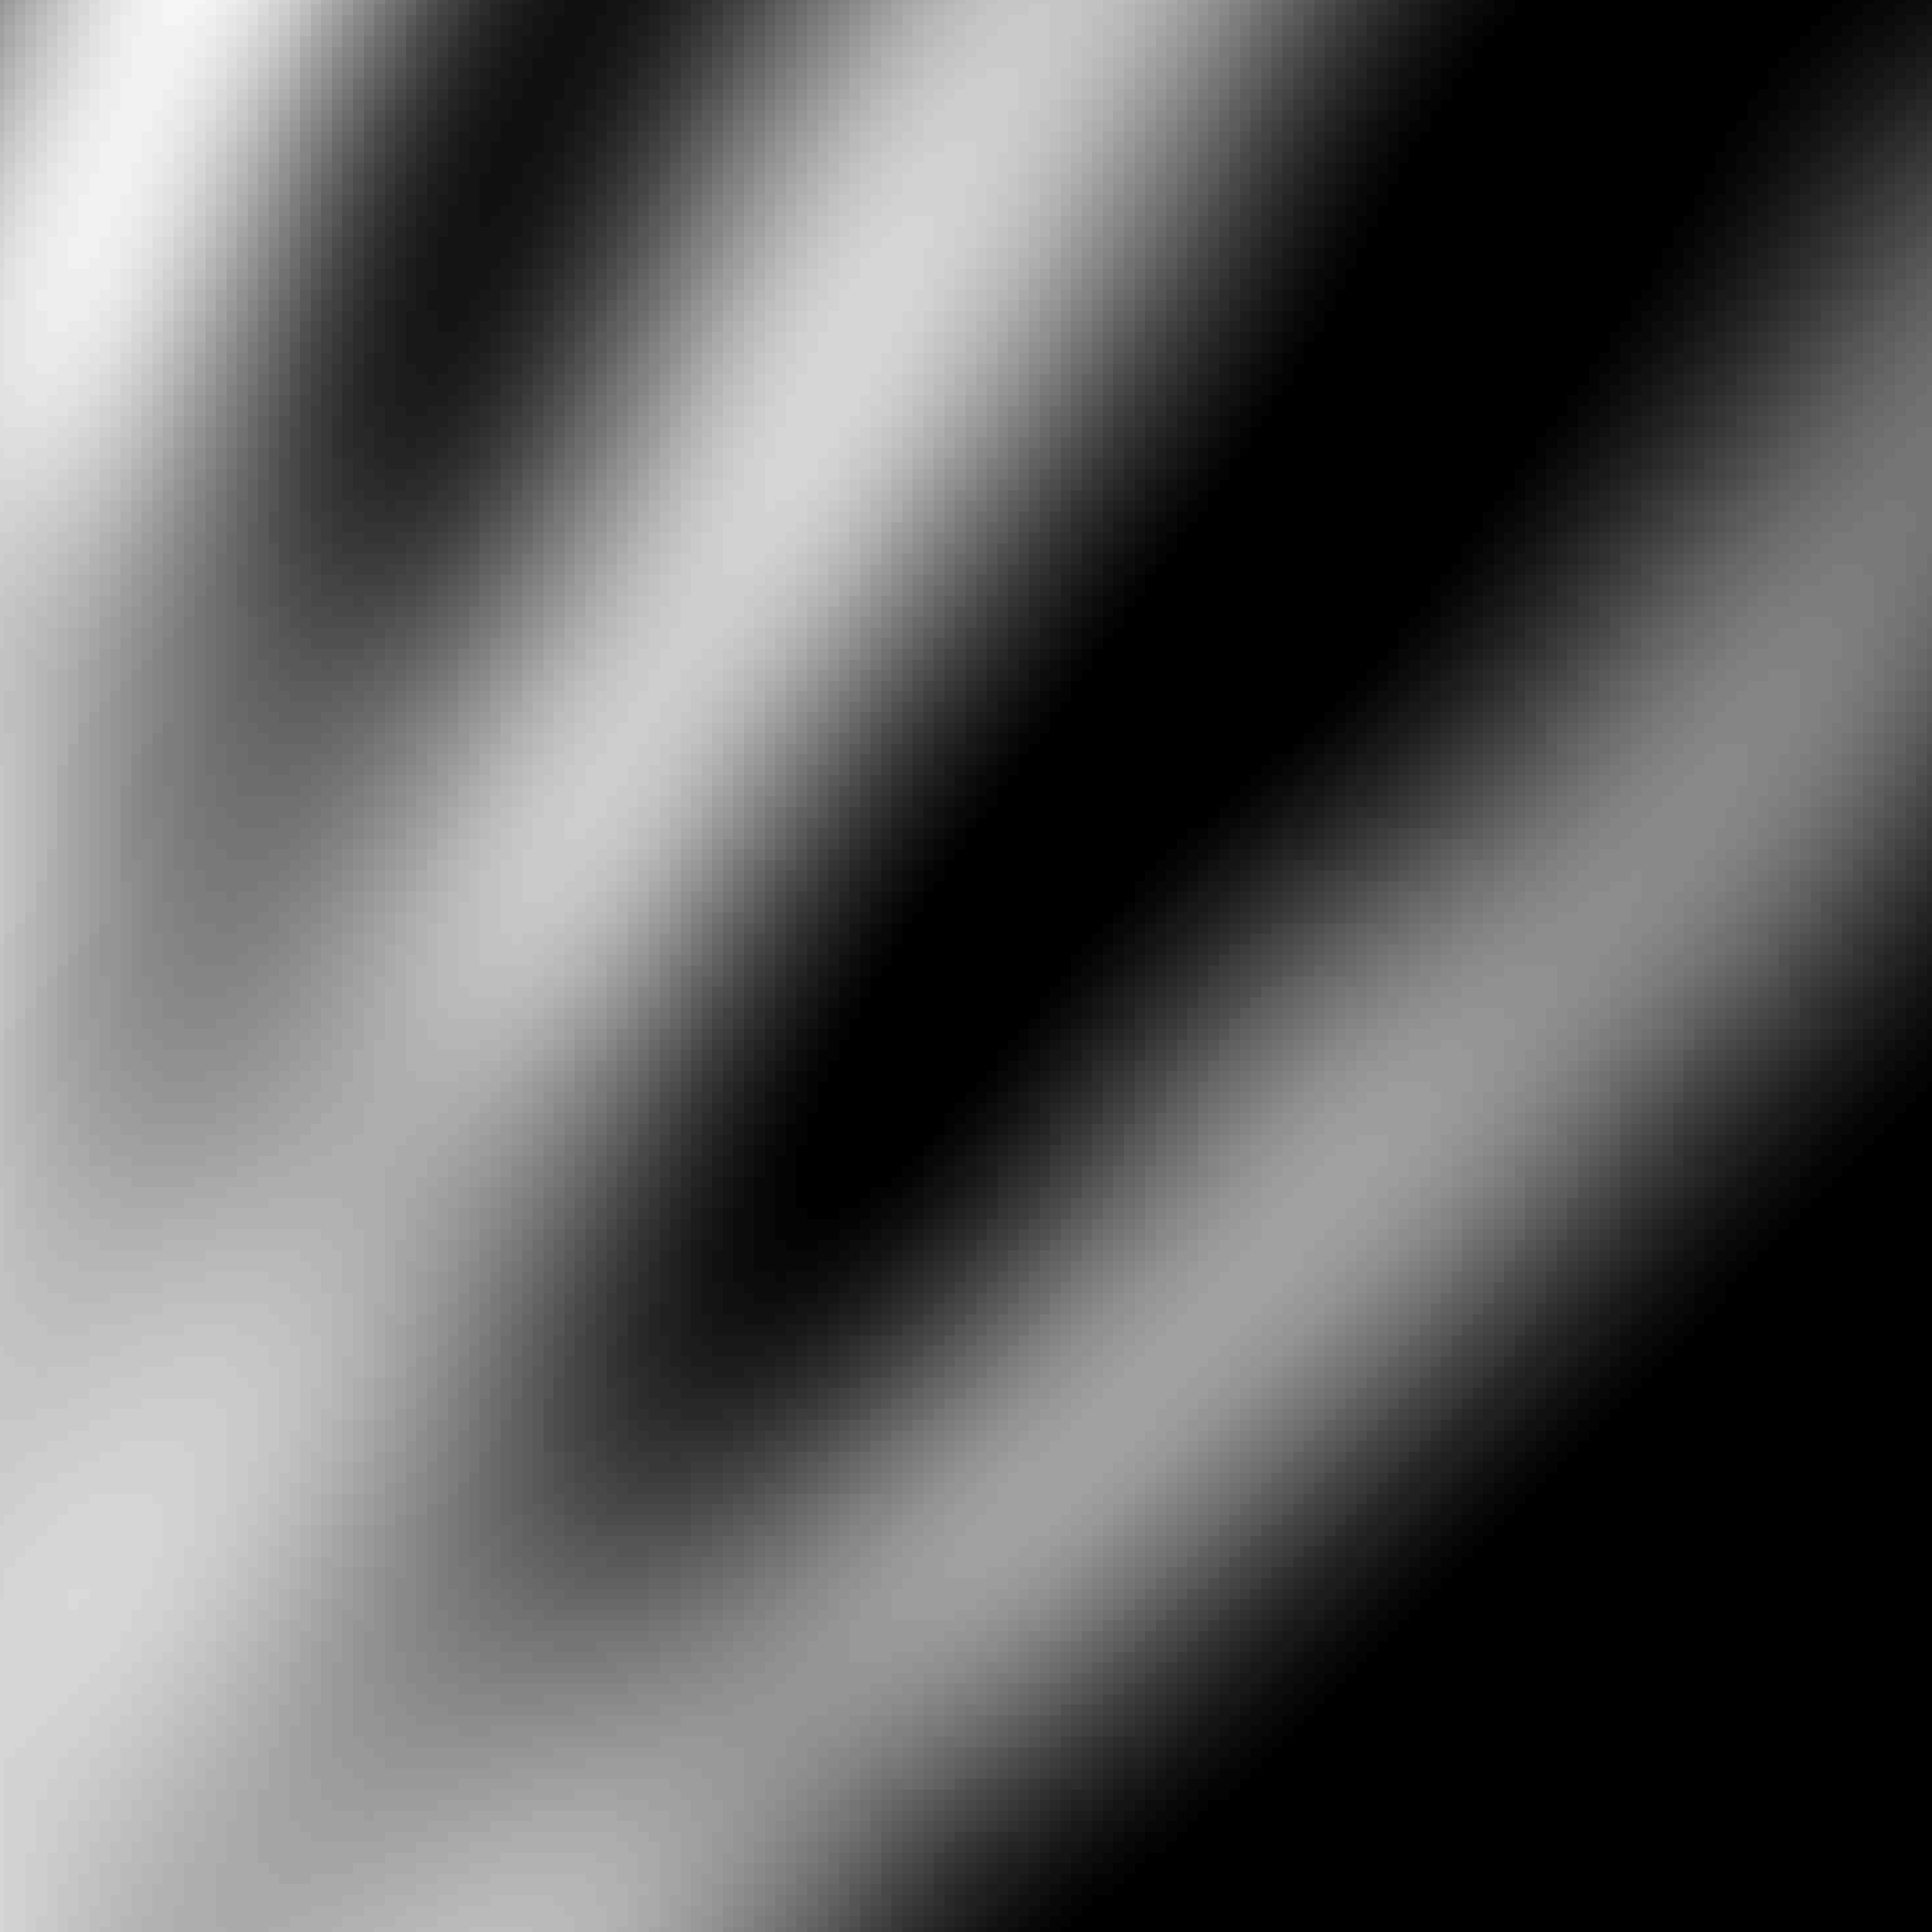
\includegraphics[width=30mm]{image-model2D-spline}}
		\end{tabular}
	\end{center}
	
	Digital images are arrays $\bfU = \R^{m_1\times m_2 \times c}$ ($c=1 \leadsto$ grey only).
	\begin{itemize}
		\item perhaps most common interpretation in image processing
	\end{itemize}
	
	\bigskip
	\pause
	
	Continuous point of view: Images are functions supported on a domain $\Omega \in \R^{2}$  $u : \Omega \to \R^c$.
	\begin{itemize}
		\item choose function space (e.g., continuous, differentiable)
		\item discretize on regular grids $\leadsto$ digital image
		\item apply operators to images (e.g., gradient in edge detection)
	\end{itemize} 
\end{frame}

\begin{frame}[fragile]\frametitle{Type of Regularization}

{\bf Classical Tikhonov} (aka weight decay) \\
$$ R(\bfW) = \hf \|\bfW\|_F^2 $$
requires elements to be small.

\bigskip

When $\bfY$ are images, also columns in $\bfW$ can be seen as images
$$ \bfw^{\top} \bfy \approx \int_{\Omega} w(\bfxi) y(\bfxi) d\bfxi. $$

{\bf General Tikhonov}: Let $\bfL$ be a given matrix \\
$$ R(\bfW) = \hf \|\bfL \bfW\|_F^2 $$
If $\bfL$ is discrete derivative operator, entries need to be smooth.

\end{frame}

\begin{frame}[fragile]\frametitle{Discretization of $\nabla^2$}
	
	Idea: Ensure classifier is smooth by using $\bfL \approx \nabla^2$.
	
	\bigskip
	\pause

Finite difference in 1D: 	Let $\bfu \in \R^{m}$ be discretization of $u: [0,1] \to \R$ on regular grid with pixel size $h=1/m$
$$ \nabla^2 u(x_j) \approx  {\frac 1 {h^2}} (-2 \bfu_{j} +  \bfu_{j-1} + \bfu_{j+1}). $$

\bigskip
\pause
Code in 1D
\begin{verbatim}
L1D = @(m,h) 1/h^2 *...
 spdiags(ones(n,1)  * [1  -2  1],-1:1,m,m)
\end{verbatim}


\bigskip
\pause

Finite difference in 2D: Let $\bfU \in \R^{m\times m}$ be discretization of $u: [0,1]^2 \to \R$ on regular grid with pixel size $h=1/m$

$$ \nabla^2 I(x_{ij}) \approx  {\frac 1 {h^2}} (-4 \bfI_{ij} + \bfI_{i-1j} + \bfI_{i+1j} + \bfI_{ij-1} + \bfI_{ij+1}). $$


\bigskip


\end{frame}


\begin{frame}[fragile]\frametitle{Discretization of $\nabla^2$}

In 2D $\quad \nabla^2 = {\frac {\partial^2}{\partial x^2}} + {\frac {\partial^2}{\partial y^2}} $


\bigskip

Use Kroneker products
$$ {\rm vec}(\bfL \bfU \bfI) = (\bfI^{\top} \otimes \bfL) {\rm vec} (\bfU). $$


Code in 2D
\begin{verbatim}
L = kron(speye(m2), L1D(m1,h1)) + ...
      kron(L1D(m2,h2),speye(m1) );
\end{verbatim}

\end{frame}

\begin{frame}[fragile]\frametitle{More about discrete $\nabla^2$}

Note that $\bfL$ can also be written as a convolution
$$ \bfL = {\frac 1 {h^2}}\ \  \begin{pmatrix} 0  &  1  &  0 \\ 1  & -4  & 1 \\ 0  & 1  & 0 \end{pmatrix} * \bfU. $$

In general - any differential operator with constant coefficients can be written
as convolution and vice versa.

\bigskip

Continuous interpretation allows re-computing a convolution kernel for different image resolutions.


\end{frame}
% section regularization_in_imaging (end)

\section{Numerical Optimization} % (fold)
\label{sec:numerical_optimization}
\begin{frame}[fragile]\frametitle{Recap: Numerical Optimization}

Require derivatives of the regularization to efficiently solve
$$ \min_{\bfW} \ \phi(\bfW) = E(\bfW) + \lambda R(\bfW) $$


\bigskip
\pause

{\bf Tip for Newton:} Use $\nabla^2 R$ as a preconditioner for the conjugate gradient
solver in the Newton iteration. 

\bigskip
\pause
\textbf{Exercise:} Setup smoothness regularizer and test it on MNIST and CIFAR-10
\end{frame}



\begin{frame}[allowframebreaks]
	\frametitle{References}
\bibliographystyle{abbrv}
 % \bibliographystyle{plainnat}
\bibliography{NumDNN}

\end{frame}

\end{document}
















